\chapter{Formalism}
\label{chap:cpv:theory}

The origin of direct \CP\ violation in weak interactions is described in 
\cref{chap:intro:sm:cp}.
This \lcnamecref{chap:cpv:theory} will present the formalism of the measurement 
of \dACP, and will enumerate the production and detection asymmetries that may 
enter.

The measurement of \ARaw, as defined in \cref{eqn:cpv:introduction:araw}, can 
be contaminated by production and detection asymmetries.
By reconstructing \LcTopKK\ and \LcToppipi\ decays from 
\decay{\PLambdab}{\PLambdac\Pmuon X}\ decays, \ARaw\ can include the effects of 
the \PLambdab/\APLambdab\ production asymmetry, the \Pmuon/\APmuon detection 
asymmetry, and the detection asymmetry of the \PLambdac\ final state 
$f$/$\bar{f}$.

The \PLambdab\ production asymmetry is predicted to be non-zero due to the \pp\ 
collision environment~\cite{PhysRevD.90.014023}.
\lhcb\ has found evidence of such an asymmetry as a function of \PLambdab\ 
rapidity~\cite{Aaij:2015fea}, shown in \cref{fig:cpv:syst:asym:lambdab}.
The two detection asymmetries are also expected to be non-zero, due to the 
known differences between the hadron/anti-hadron and muon/anti-muon 
cross-sections with matter~\cite{PDG2014}, as shown in 
\cref{fig:cpv:syst:asym:xsecs}.
The final state detection asymmetry can be broken down into two terms: one due 
to the detection asymmetry of the proton; and another due to the detection 
asymmetry of the \KmKp pair and the \pimpip\ pair.
If the meson kinematics are equal within a given mode, for example if the 
\PKminus kinematics are identical to those of the \PKplus\ in the \pKK\ data, 
then the final state asymmetry reduces to the proton detection asymmetry.

\begin{figure}
  \centering
  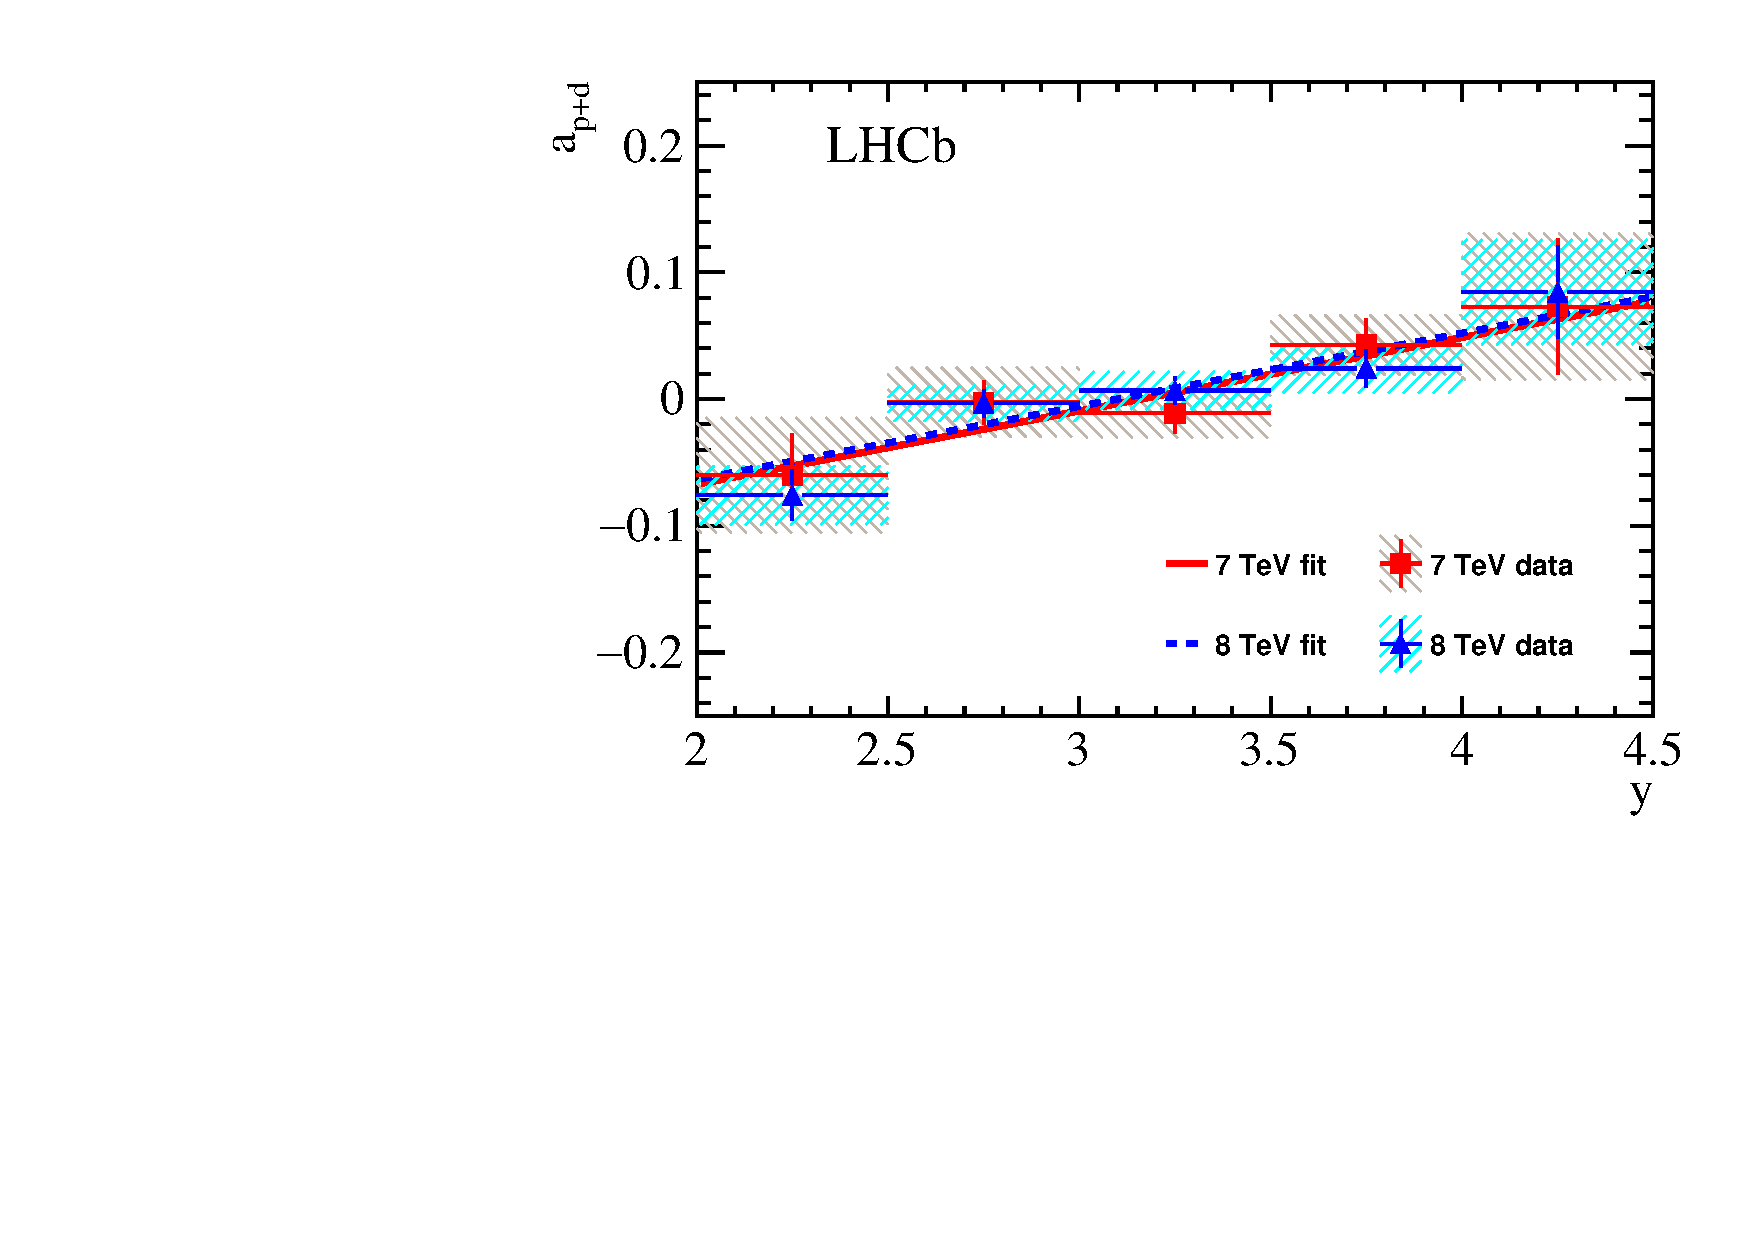
\includegraphics[width=0.75\textwidth]{cpv/systematics/lambdab_production_asymmetry_y}
  \caption{%
    Asymmetry of \PLambdab\ production as a function of \PLambdab\ rapidity.
    The uncertainties on the data points are statistical, whilst the hatched 
    bands include both the statistical and systematic uncertainties.
  }
  \label{fig:cpv:syst:asym:lambdab}
\end{figure}

\begin{figure}
  \begin{subfigure}{0.5\textwidth}
    \centering
    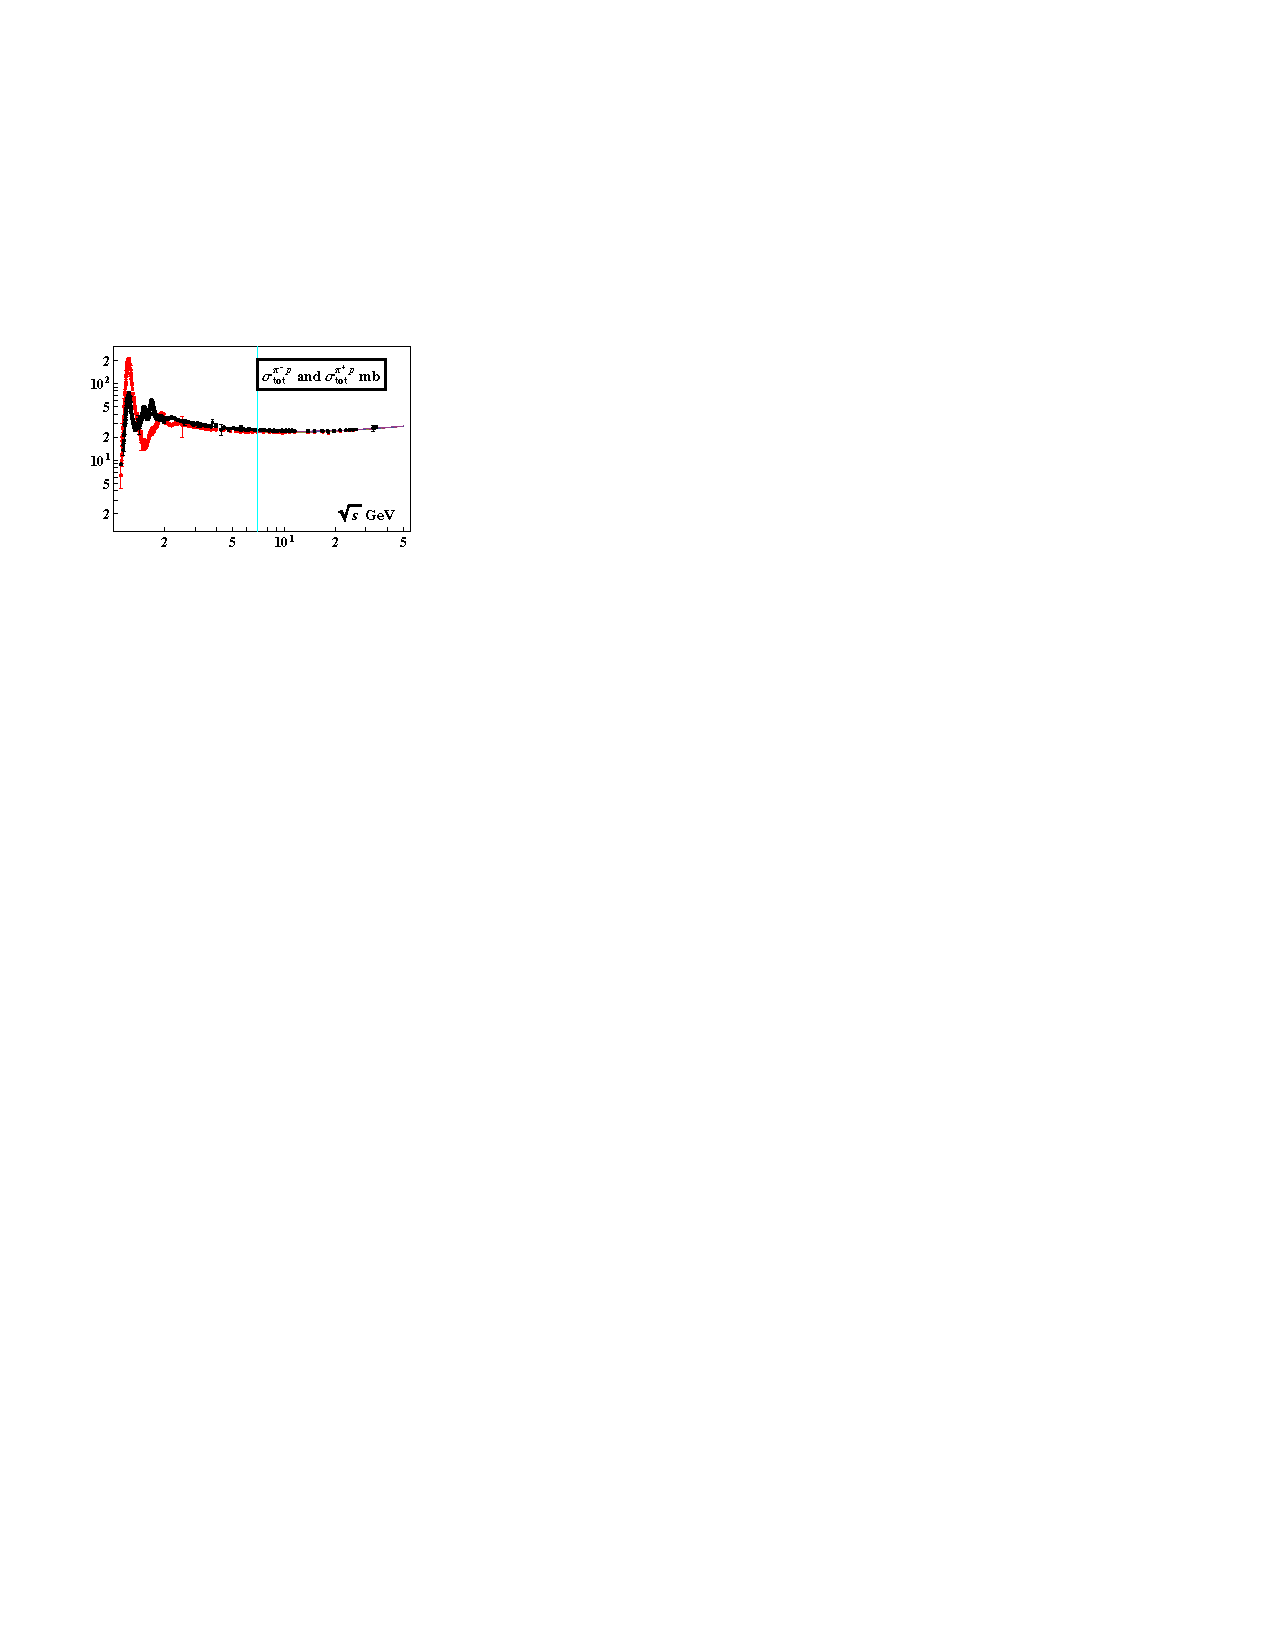
\includegraphics[width=\textwidth]{cpv/systematics/pion_proton_cross_sections}
    \caption{\decay{\Ppi\Pproton}{X}}
    \label{fig:cpv:syst:asym:xsecs:pion}
  \end{subfigure}
  \begin{subfigure}{0.5\textwidth}
    \centering
    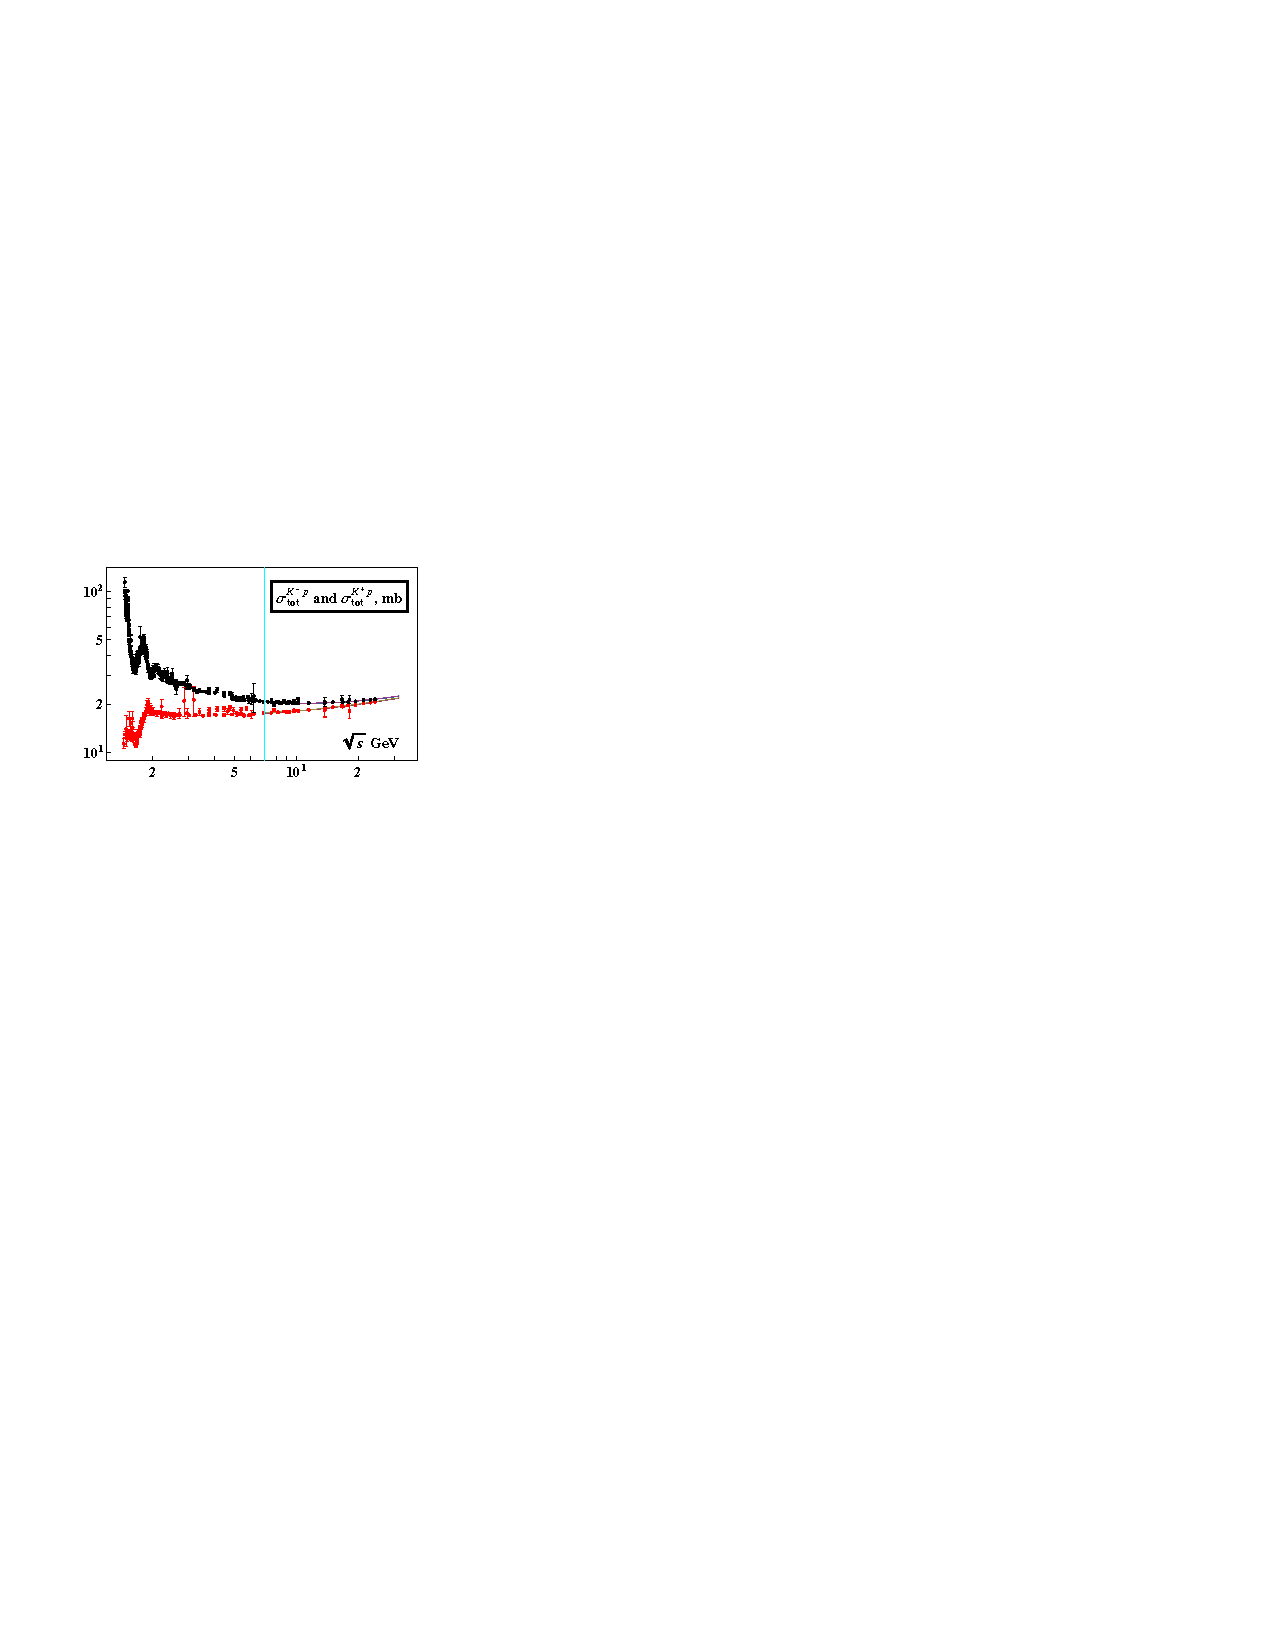
\includegraphics[width=\textwidth]{cpv/systematics/kaon_proton_cross_sections}
    \caption{\decay{\PK\Pproton}{X}}
    \label{fig:cpv:syst:asym:xsecs:kaon}
  \end{subfigure}
  \begin{subfigure}{0.5\textwidth}
    \centering
    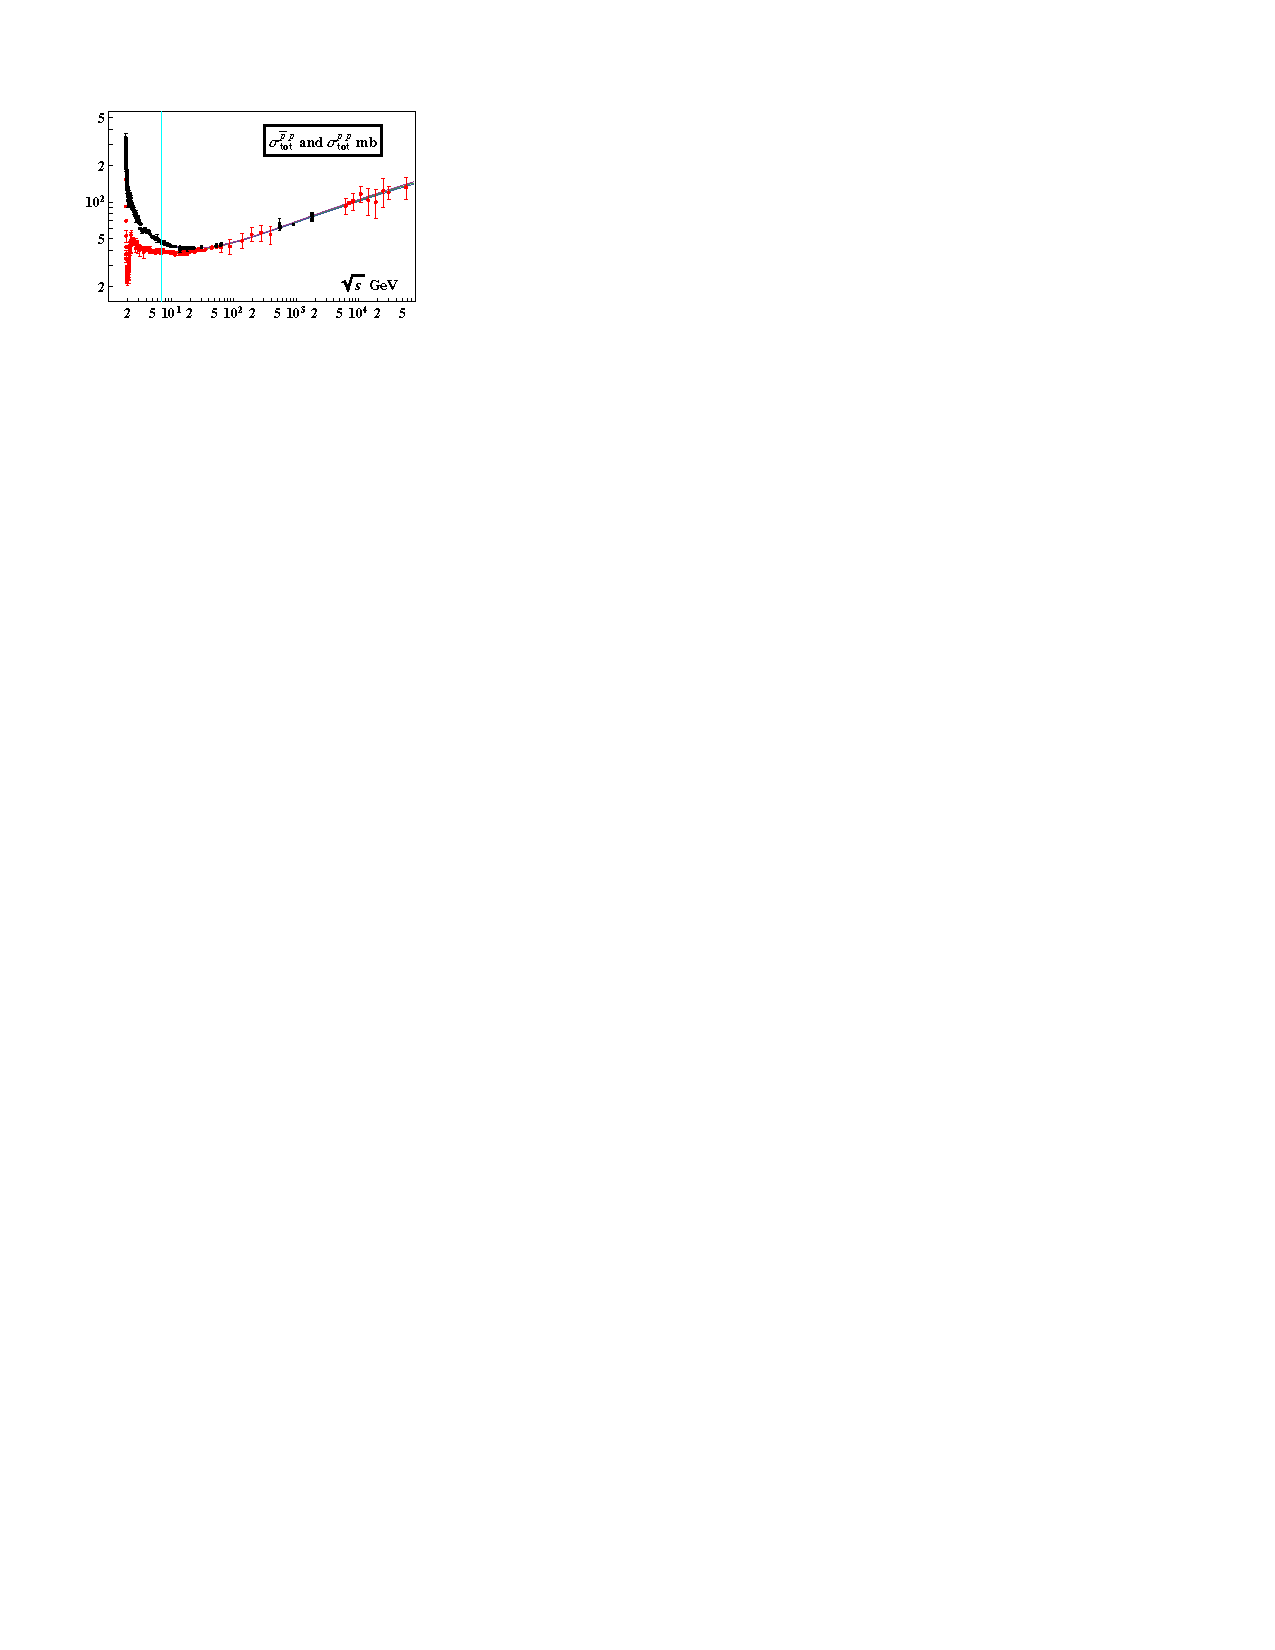
\includegraphics[width=\textwidth]{cpv/systematics/proton_proton_cross_sections}
    \caption{\decay{\Pproton\Pproton}{X}}
    \label{fig:cpv:syst:asym:xsecs:proton}
  \end{subfigure}
  \caption{%
    Cross-sections of $h^{\mp}\Pproton \to \text{anything}$~\cite{PDG2014}.
    Each curve shows the hadronic cross-section with proton targets as a 
    function of \sqrts, with the red curve showing the cross-section for the 
    `matter' hadron (\PKplus, \Ppiplus, \Pproton) and the black curve showing 
    that for the `antimatter' hadron (\PKminus, \Ppiminus, \APproton).
  }
  \label{fig:cpv:syst:asym:xsecs}
\end{figure}

Both the \PLambdab\ production and the muon detection asymmetries should be 
independent of the \PLambdac\ final state, given the same \PLambdac\ 
kinematics.
Different acceptance efficiencies between \pKK\ and \ppipi\ can create unequal 
\PLambdac\ kinematics, but the kinematics can be weighted to equalise them 
between the modes.

It will now be shown how the background asymmetries entering \ARaw\ can be 
removed in the difference \dACP\@.
The number of reconstructed \LcTof\ decays can be expressed as the product of 
several effective probabilities
\begin{equation}
  N(f) = \prob(\PLambdab)\cdot
         \Gamma(\LbToLcmuX)\cdot
         \Gamma(\LcTof)\cdot
         \eff(\Pmuon)\cdot
         \eff(f),
  \label{eqn:cpv:theory:yield}
\end{equation}
where $\prob(\PLambdab)$ is the probability of producing a $\PLambdab$ baryon 
given a \pp\ collision, and $\eff(\Pmuon)$ and $\eff(f)$ are the muon and 
$\PLambdac$ final-state detection efficiencies.
A similar expression exists for $N(\bar{f})$, where are parameters are replaced 
by their charge conjugates.
% TODO can we back up this assumption?
It is assumed that the \LbToLcmuX decay is \CP-symmetric, but that all other 
factors may not be, for example $\eff(\Pmuon) \neq \eff(\APmuon)$.

To express \ARaw\ in terms of its component asymmetries, the notation of a 
general asymmetry parameter $X$ is defined, which describes the asymmetry 
between two quantities $x$ and $\bar{x}$
\begin{equation}
  X = \frac{x - \bar{x}}{x + \bar{x}}.
  \label{eqn:cpv:theory:generic_asym}
\end{equation}
This can be rearranged as
\begin{align}
  x &= \frac{1}{2}(x + \bar{x})(1 + X),\label{eqn:cpv:theory:asym_form_one}\\
  \bar{x} &= \frac{1}{2}(x + \bar{x})(1 - X).\label{eqn:cpv:theory:asym_form_two}
\end{align}
An asymmetry parameter like that in \cref{eqn:cpv:theory:generic_asym} can be defined for each of the relevant terms in 
\cref{eqn:cpv:theory:yield}
\begin{align*}
  \APLb(f) &= \frac{%
    \prob(\PLambdab) - \prob(\APLambdab)
  }{%
    \prob(\PLambdab) + \prob(\APLambdab)
  },\\
  \ADmu(f) &= \frac{%
    \eff(\Pmuon) - \eff(\APmuon)
  }{%
    \eff(\Pmuon) + \eff(\APmuon)
  },\\
  \ADf(f)  &= \frac{%
    \eff(f) - \eff(\bar{f})
  }{%
    \eff(f) + \eff(\bar{f})
  },
\end{align*}
and the asymmetry in $\Gamma(\LcTof)$ is \ACP as in 
\cref{eqn:cpv:introduction:acp}.
Each parameter is, at least implicitly, dependent on the detected \PLambdac\ 
final state, as each parameter can vary in quantities that may also vary 
between \PLambdac\ decay modes.
Substituting in Equation~\ref{eqn:cpv:theory:yield} to 
Equation~\ref{eqn:cpv:introduction:araw}
\begin{equation*}
  \ARaw(f) = \frac{%
    \prob(\PLambdab)\Gamma(f)\eff(\Pmuon)\eff(f) - 
    \prob(\APLambdab)\Gamma(\bar{f})\eff(\APmuon)\eff(\bar{f})
  }{%
    \prob(\PLambdab)\Gamma(f)\eff(\Pmuon)\eff(f) + 
    \prob(\APLambdab)\Gamma(\bar{f})\eff(\APmuon)\eff(\bar{f})
  },
\end{equation*}
and then substituting each quantity for its equivalent form as in 
\cref{eqn:cpv:theory:asym_form_one,eqn:cpv:theory:asym_form_two}, all factors 
of $\sfrac{1}{2}$ and all factors of the form $(x - \bar{x})$ cancel, leaving
\begin{equation}
  \ARaw(f) = \frac{Y}{Z}.
\end{equation}
where (dropping the final state parameter temporarily for compactness)
\begin{align}
  Y = \APLb\ADmu\ADf &+ \APLb\ADmu\ACP + \APLb\ADf\ACP + \ADmu\ADf\ACP \nonumber\\
                     &+ \APLb +  \ADmu + \ADf + \ACP,
\end{align}
and
\begin{align}
  Z = 1 &+ \APLb\ADmu + \APLb\ADf + \APLb\ACP + \ADmu\ADf + \ADmu\ACP \nonumber\\
        &+ \ADf\ACP + \APLb\ADmu\ADf\ACP.
\end{align}
Assuming that the individual asymmetries are small, of the order of 
\SI{1}{\percent}, the product of two or more asymmetries is negligible with 
respect to the leading order, and so
\begin{equation}
  \ARaw(f) \approx \ACP(f) + \APLb(f) + \ADmu(f) + \ADf(f).
  \label{eqn:cpv:theory:araw_approx}
\end{equation}
By assuming that these background asymmetries are mode-independent, that is to 
say $\AD(f) = \AD(g)$ and $\AP(f) = \AP(g)$, the difference between \ARaw\ for 
the \pKK\ and \ppipi\ will only have contributions from \ACP
\begin{align}
  \dACP &= \ARaw(\pKK) - \ARaw(\ppipi),\label{eqn:cpv:theory:dacp}\\
        &\approx \ACP(\pKK) - \ACP(\ppipi)\nonumber.
\end{align}

The assumption that the production and detection asymmetries in 
\cref{eqn:cpv:theory:araw_approx} are mode independent is not true in general.
This can been seen by first making a weaker assumption that the background 
asymmetries are dependent only on the kinematics of the representative 
particles.
Different final states will in general have different acceptance, 
reconstruction and selection efficiencies as a function of \PLambdac\ 
kinematics.
The kinematics of the \PLambdac\ are correlated to those of the muon and the 
\PLambdab, and so two samples with different \PLambdac\ kinematics will likely 
also have different \PLambdab\ and muon kinematics.
Hence, there can still be net production and detection asymmetries in \dACP\@.

The assumption that the background asymmetries depend only on particle 
kinematics is not unreasonable.
The production asymmetry, for example, is a difference in cross-sections, which 
are usually parameterised by the kinematics of the produced particle (\pT\ and 
either \Eta or rapidity).
Similarly, a detection asymmetry describes the differences of material 
interactions between matter and antimatter, and these are dependent on the 
momentum of the particle in question and, assuming a non-uniform material 
distribution, its flight path.

As it is not given that the \PLambdac\ kinematics are equal between \LcTopKK\ 
and \LcToppipi\ decays in the data, the data can be weighted to equalise the 
\PLambdac\ kinematics.
The background asymmetries \AP\ and \ADmu\ will then cancel in the difference 
\dACP\@.
The proton kinematics will not necessarily agree after such a weighting, as the 
energy release in the \pKK\ and \ppipi\ decays is different.
These considerations govern the analysis strategy: measure the number of 
\PLambdac\ candidates in the \pKK\ and \ppipi\ samples after weighting them 
such that the \PLambdac\ kinematics look alike, such that the \PLambdab\ and 
\Pmuon kinematics also agree.
Additional weighting may be required to equalise the proton kinematics.

\section{Decay phase space}
\label{chap:cpv:theory:phsp}

The phase space of a decay is the set of variables which fully parameterises 
all possible dynamics.
For the decay of a pseudo-scalar to three pseudo-scalars, such as 
\decay{\PDzero}{\PKshort\Ppiplus\Ppiminus}, the spin symmetry of the final 
allows for the phase space to be fully parameterised by two variables.
These are usually taken to be two child-pair squared masses, which can 
visualised as a Dalitz plot.
In the case of \LcTophh, the spin \sfrac{1}{2} of the proton means that 
three-body system is no longer rotationally symmetric, and three additional 
variables are required to describe the phase space.

For a meaningful comparison of the measurement of \dACP\ with theoretical 
predictions, which are not presently available, the efficiency of the 
\PLambdac\ selection across the five-dimensional phase space must be known.
The definition of ``selection'' includes the effects of the \lhcb\ acceptance 
and the trigger, stripping, and offline requirements.
The efficiency model can either be provided to theorists so that they can apply 
the same efficiencies to their phase space models, or it can be used to correct 
the data before the \dACP\ measurement is made.

The five dimensions of the phase space is defined here in a similar way to the 
\LcTopKpi\ amplitude analysis performed by the \esno\ 
collaboration~\cite{Aitala:1999uq}.
This defines two child-pair square masses, of the proton and oppositely-charged 
child \msqphm\ and of the two opposite-sign pseudo-scalars \msqhh, and three 
decay angles.
The child-pair square masses are invariant under Lorentz transformations, but 
the decay angles are not and so a definition of the frame in which they are 
computed is required.

The \esno\ analysis defines a coordinate system in the \PLambdac\ rest frame.
The $z$-axis, also called the quantisation axis or polarisation axis \polzlcp, 
is perpendicular to the plane of production
\begin{equation}
  z = \polzlcp = \phatbeam \times \phatlcp,
\end{equation}
where \phatbeam\ is the direction of the beam\footnotemark\ and \phatlcp\ is 
the direction of the \PLambdac\ measured in the laboratory frame.
\footnotetext{%
  E791 was a fixed-target experiment, colliding a \SI{500}{\GeVc} pion beam 
  with metal foils.
}
The $x$-axis of the \PLambdac\ rest frame is \phatlcp.
As the \PLambdac\ candidates in this analysis are not produced directly from 
the \pp\ collision but in the decays of \PLambdab\ baryons, here the `beam 
direction' is defined as the direction of the \PLambdab\ momentum vector, which 
is equal to the direction vector pointing from the \pp\ primary vertex 
$v_{\pp}$ to the $\PLambdac\Pmuon$ vertex $v_{\PLambdac\Pmuon}$
\begin{equation}
  \phatbeam = \phatlbz = v_{\PLambdac\Pmuon} - v_{\pp}.
\end{equation}
With this coordinate system and inertial frame, the three decay angles are 
defined as:
\begin{enumerate}
  \item The angle \thetap\ between the proton momentum vector and the $z$-axis;
  \item The angle \phip\ between the proton momentum vector and the $x$-axis; 
    and
  \item The angle \phihh\ between the plane containing the proton momentum 
    vector and the $z$-axis and the plane containing the two pseudo-scalar 
    meson momentum vectors.
\end{enumerate}
These definition are illustrated in \cref{fig:cpv:theory:phsp:angles}

The distributions of the five phase space variables will be presented in 
\cref{chap:cpv:phsp}, along with the evaluation of the efficiency as a function 
of the position in phase space.

\begin{figure}
  \begin{subfigure}{0.5\textwidth}
    \resizebox{\textwidth}{!}{%
      % Rotation of the axes wrt the viewer
% syntax: \tdplotsetdisplay{\theta_d}{\phi_d}
\tdplotsetmaincoords{70}{110}

% Define proton coordinates
\pgfmathsetmacro{\rp}{.8}
\pgfmathsetmacro{\angthetap}{60}
\pgfmathsetmacro{\angphip}{50}

% Define Kpi coordinates
\pgfmathsetmacro{\rKpi}{.4}
\pgfmathsetmacro{\thetaKpi}{80}
\pgfmathsetmacro{\phiKpi}{340}

% Start a TikZ picture, using the tdplot_main_coords system
% tdplot provides the coordinate transformation
\begin{tikzpicture}[scale=4,tdplot_main_coords]

% Define the origin
\coordinate (O) at (0,0,0);

% Create a point P with coordinates r, theta, and phi
% I think this is similar to \coordinate, but also transform the vector
% in to the rotated coordinate system
\tdplotsetcoord{P}{\rp}{\angthetap}{\angphip}
\tdplotsetcoord{Kpi}{\rKpi}{\thetaKpi}{\phiKpi}

% Draw main coordinate axes
% The anchor key relates to the positioning of the label
% South is towards the bottom of the diagram, east is to the left
\draw[thick,->] (0,0,0) -- (1.0,0,0) node[anchor=north west]{
  $x = \hat{p}_{\PLambdac}$
};
\draw[thick,->] (0,0,0) -- (0,0.5,0) node[anchor=north west]{
  $y$
};
\draw[thick,->] (0,0,0) -- (0,0,0.5) node[anchor=south]{
  $z = \polzlcp = \phatlbz \times \phatlcp$
};

% Draw a vector from origin to point P
% The -stealth' option is the type of arrowhead
\draw[-stealth',color=red] (O) -- (P) node[anchor=west]{\Pproton};
\draw[-stealth',color=red] (O) -- (Kpi) node[anchor=east]{\hmhp};

% Draw projection of vector on to xy plane, and a connecting line
\draw[dashed, color=red] (O) -- (Pxy);
\draw[dashed, color=red] (P) -- (Pxy);

% Draw angle phi of xy projection
% {} arguments are center point, radius, angle-from, angle-to, options, label
% [] arguments are coordinate frame, draw options
\tdplotdrawarc{(O)}{0.25}{0}{\angphip}{anchor=north}{\phip}

%set the rotated coordinate system so the x'-y' plane lies within the
%"theta plane" of the main coordinate system
%syntax: \tdplotsetthetaplanecoords{\phi}
% Rotate the "theta plane" (xz) by phi around z
\tdplotsetthetaplanecoords{\angphip}

% Draw arc in rotated system
\tdplotdrawarc[tdplot_rotated_coords]{(0,0,0)}{0.35}{0}{\angthetap}{anchor=south west}{\thetap}

\end{tikzpicture}

    }
  \end{subfigure}
  \begin{subfigure}{0.5\textwidth}
    \resizebox{\textwidth}{!}{%
      % Rotation of the axes about x-axis, then about z-axis
% We align the x-axis with the negative proton momentum
\tdplotsetmaincoords{0}{0}

% Define proton coordinates
\pgfmathsetmacro{\rp}{0.7}
\pgfmathsetmacro{\angthetap}{90}
\pgfmathsetmacro{\angphip}{180}

% Polarisation axis 'coordinates'
\pgfmathsetmacro{\rpol}{0.7}
\pgfmathsetmacro{\thetapol}{90}
\pgfmathsetmacro{\phipol}{135}

% Define h+h- coordinates
\pgfmathsetmacro{\rKpi}{.4}
\pgfmathsetmacro{\thetaKpi}{80}
\pgfmathsetmacro{\phiKpi}{340}

% Define h+ coordinates
\pgfmathsetmacro{\rhp}{.4}
\pgfmathsetmacro{\thetahp}{90}
\pgfmathsetmacro{\phihp}{-20}

% Define h+ coordinates
\pgfmathsetmacro{\rhm}{.6}
\pgfmathsetmacro{\thetahm}{90}
\pgfmathsetmacro{\phihm}{30}

% Start a TikZ picture, using the tdplot_main_coords system
% tdplot provides the coordinate transformation
\begin{tikzpicture}[scale=4,tdplot_main_coords]

% Define the origin
\coordinate (O) at (0,0,0);

% Create a point P with coordinates r, theta, and phi
% I think this is similar to \coordinate, but also transform the vector
% in to the rotated coordinate system
\tdplotsetcoord{P}{\rp}{\angthetap}{\angphip}
\tdplotsetcoord{Hp}{\rhp}{\thetahp}{\phihp}
\tdplotsetcoord{Hm}{\rhm}{\thetahm}{\phihm}
\tdplotsetcoord{Pol}{\rpol}{\thetapol}{\phipol}
\tdplotsetcoord{Kpi}{\rKpi}{\thetaKpi}{\phiKpi}

% h+h- plane parameters
\pgfmathsetmacro{\hhHeight}{1}
\pgfmathsetmacro{\hhWidth}{0.7}
\pgfmathsetmacro{\hhSkew}{30}
\pgfmathsetmacro{\hhSkewWidth}{tan(\hhSkew)*\hhHeight}
\coordinate (hhOrigin) at ($(-\hhSkewWidth/2,-0.5)$);

% Draw planes before anything else, as fill would cover them
% Proton-z plane
\filldraw[semithick,black,fill=white] ($(P)-(0.1,0.6)$) rectangle (0,0.8);
% h+h- plane
\filldraw[semithick,black,fill=white] (hhOrigin)
  -- ($(hhOrigin)+(\hhSkewWidth, \hhHeight)$)
  -- ($(hhOrigin)+(\hhSkewWidth+\hhWidth,\hhHeight)$)
  -- ($(hhOrigin)+(\hhWidth, 0)$)
  % Close the path
  -- cycle;
% Angle between planes
% \draw[dotted] (hhOrigin) -- ($(hhOrigin)+(0, \hhHeight)$);
\tdplotdrawarc[dotted,very thick]{(O)}{0.5}{90}{
  90-\hhSkew
}{anchor=south west}{\Large$2\pi - \phihh$}

% Draw main coordinate axes
% The anchor key relates to the positioning of the label
% South is towards the bottom of the diagram, east is to the left
% \draw[thick,->] (O) -- (1,0,0) node[anchor=north west]{
%   $x = \hat{p}_{\PLambdac}$
% };
% \draw[thick,->] (O) -- (0,1,0) node[anchor=north west]{
%   $y$
% };

% Proton
\draw[-stealth',color=red] (O) -- (P) node[anchor=south]{\Large\Pproton};
% Polarisation axis
\draw[thick,->] (O) -- (Pol) node[anchor=south]{
  \Large$z = \polzlcp$
};

% h+
\draw[-stealth',color=red] (O) -- (Hp) node[anchor=north]{\Large\Php};
% h-
\draw[-stealth',color=red] (O) -- (Hm) node[anchor=south]{\Large\Phm};

% Draw projection of vector on to xy plane, and a connecting line
% \draw[dashed, color=red] (O) -- (Pxy);
% \draw[dashed, color=red] (P) -- (Pxy);

% Draw angle phi of xy projection
% {} arguments are center point, radius, angle-from, angle-to, options, label
% [] arguments are coordinate frame, draw options
\tdplotdrawarc{(O)}{0.25}{\angphip}{\phipol}{anchor=east}{\Large\thetap}

%set the rotated coordinate system so the x'-y' plane lies within the
%"theta plane" of the main coordinate system
%syntax: \tdplotsetthetaplanecoords{\phi}
% Rotate the "theta plane" (xz) by phi around z
% \tdplotsetthetaplanecoords{\angphip}

% Draw arc in rotated system
% \tdplotdrawarc[tdplot_rotated_coords]{(0,0,0)}{0.35}{0}{\angthetap}{anchor=south 
% west}{$\theta_{p}$}

\end{tikzpicture}

    }
  \end{subfigure}
  \caption{%
    Definition of inertial reference frame axes and \LcTophh\ phase space decay 
    angles.
    Adapted from Figure~1 in the \esno\ \LcTopKpi\ amplitude analysis 
    paper~\cite{Aitala:1999uq}.
  }
  \label{fig:cpv:theory:phsp:angles}
\end{figure}
